%%%%%%%%%%%%%%%%%%%%%%%%%%%%%%%%%%%%%%%%%%%%%%%%%%%%%%%%%%%%%%%%%%%%%%%%%%%%%%%
%%                                                    DATA SIMULATION SELECTION
%%%%%%%%%%%%%%%%%%%%%%%%%%%%%%%%%%%%%%%%%%%%%%%%%%%%%%%%%%%%%%%%%%%%%%%%%%%%%%%
%%                                    about the samples, MC Generation and cuts 



%______________________________________________________________________________
%                                                Daten Simulation und Selektion 
\chapter{Daten, Simulation \& Selektion}

\begin{quote}
    The abstract come last
\end{quote}



%______________________________________________________________________________
%                                                                         Daten 
\section{Daten}
\label{data_sim_selection:data}

\begin{itemize}
    \item \sout{Daten von 2012}
    \item \sout{Parameter: Energie, Bunchespacing, Perioden}
    \item HV-Problem Anfang des Jahres
\end{itemize}

Die Daten, die dieser Arbeit zugrunde liegen, wurden vom ATLAS-Detektor im Jahr
2012 bei erstmalig $8 \TeV$ Schwerpunktsenergie aufgenommen. Der \ac{LHC} wird
mit Paketen von Protonen, sogenannte Bunches (vom engl. Bunch: Bündel) gefüllt,
die für einige Stunden im Beschleuniger zirkulieren\footnote{weitere Details:
siehe Kapitel \ref{}}.
Eine solche Füllung steht für identische Einstellungen des Beschleunigers bzw.
Detektors und wird in ATLAS mit einer fortlaufenden Nummer identifiziert.
Die Füllungs-Nummern größerer Perioden konstanter Bedingungen, wie das zu der
Zeit implementierte Trigger-Menü oder globale \ac{LHC} Parameter, werden dann
mit einem Buchstaben zusammengefasst (Periode A, B, ...).

Der vorliegende Datensatz wurde in der Zeit zwischen dem 04. April 2012 und dem
16. Dezember 2012 aufgenommen und umfasst 10 Perioden, die einer integrierten
Gesamtluminosität von $20.3 \fb^{-1}$ entsprechen\footnote{nach Anwenung der
\ac{GRL} (siehe Kapitel \ref{})} (siehe Abbildung \ref{fig:lumi}). Der Detektor
wurde hierbei in einer Konfiguration betrieben, die einen zeitlichen Abstand
zwischen den Teilchen-Paketen von $50\:\nano\second$ gewährleistet, woraus eine
instantane Luminosität\footnote{Erläuterungen zur Messung der Luminosität in
ATLAS finden sich in Kapitel \ref{}} von bis zu
$7.73 \cdot 10^{-33} \centi\meter^{-2}\second^{-1}$ resultiert.

Eine hohe instantane Luminosität verspricht eine große Rate interessanter
Ereignisse, jedoch bedingt sie auch viele unerwünschte Neben-Ereignisse,
vorwiegend aus inelastischen Streuprozessen, die einen signifikanten Einfluss
auf die Messung nehmen können. Dieser Effekt wird als \textit{Pile-Up}
bezeichnet und ist in Abbildung \ref{fig:pileup} illustriert.

\begin{figure}
    \begin{minipage}[b]{0.48\textwidth}
        \centering
        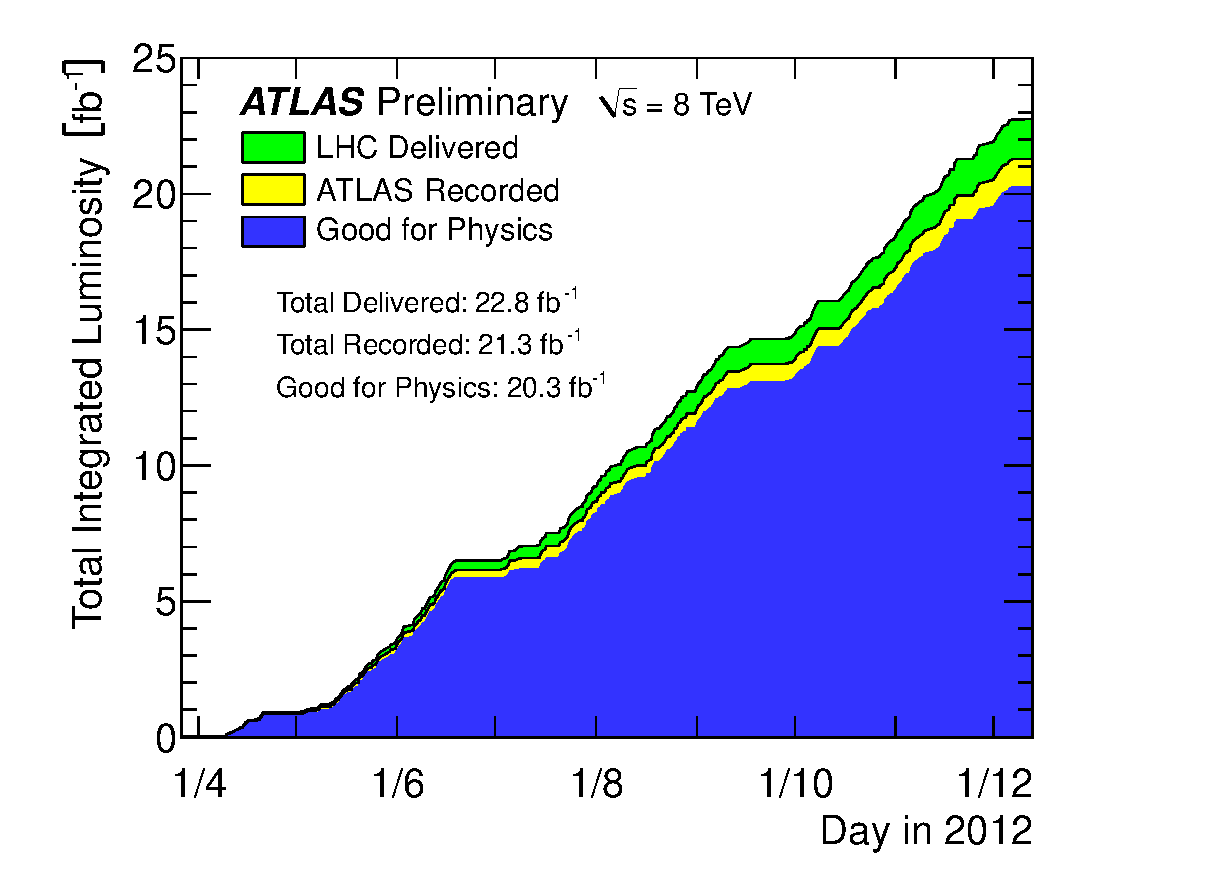
\includegraphics[width=1.\textwidth]{plots/lumi}
        \captionsetup{format=plain}
        \caption{Verfügbare, aufgezeichnete und validierte integrierte
            Luminosität aufgetragen gegen die Zeit innerhalb der Messkampange}
        \label{fig:lumi}
    \end{minipage}
    \hfill
    \begin{minipage}[b]{0.48\textwidth}
        \centering
        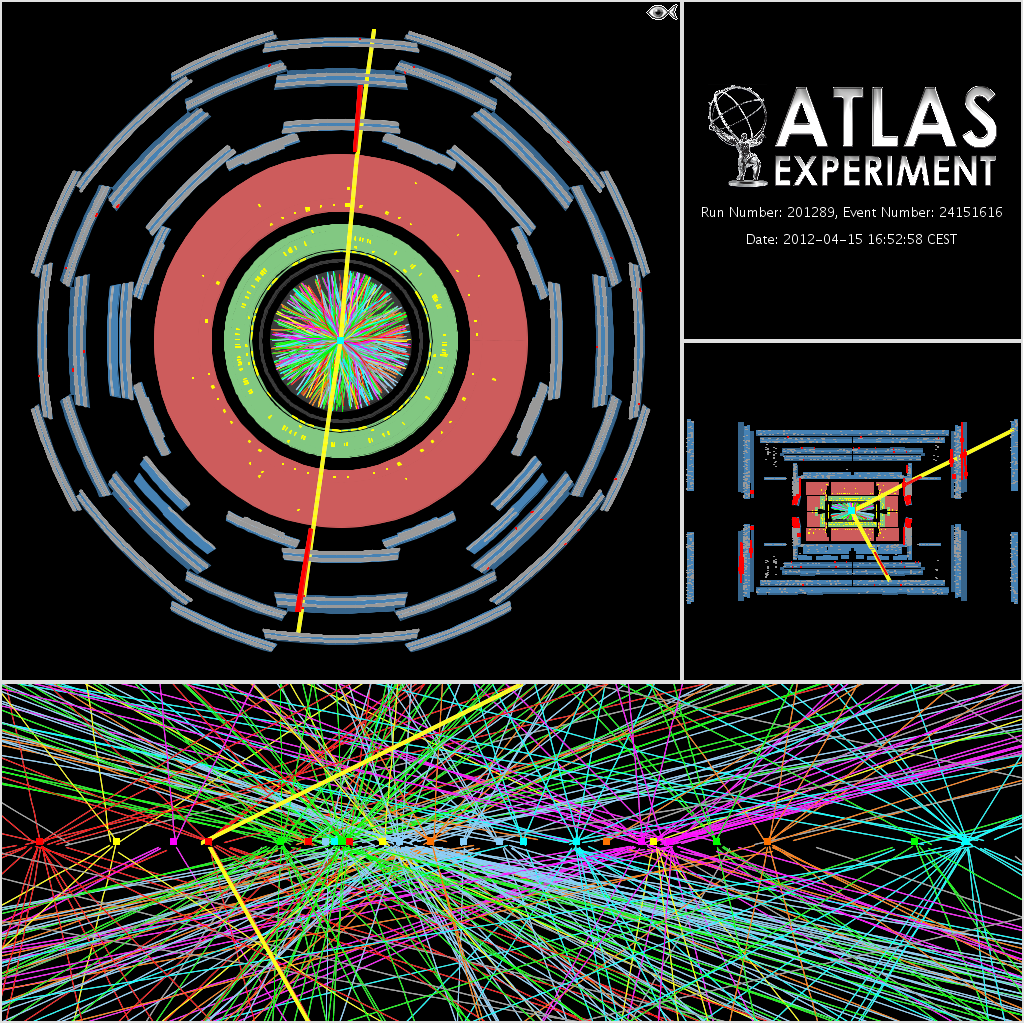
\includegraphics[width=1.\textwidth]{img/pileup}
        \captionsetup{format=plain}
        \caption{Ereignisse mit $Z \rightarrow \mu\mu$ Kandidat und hohem
            Pile-Up. 25 rekonstruierte Vertizes.}
        \label{fig:pileup}
    \end{minipage}
\end{figure}

HV-Problem \development



%______________________________________________________________________________
%                                                                    Simulation
\section{Simulation}
\label{data_sim_selection:simulation}

\begin{itemize}
    \item \sout{Motivation für Simulation (Theorie-Vorhersage)}
    \item \sout{Mehrschrittiges Prinzip}
    \item \sout{Eventgeneration (Matrixelemente, Fragmentation,...)}
    \item \sout{Detektorsimulation (+ Ausgabeformat)}
    \item \sout{Nötige Korrekturen (Pileup, Effizienzen, Smearing, kFaktors)}
    \item Übersicht und kurze(!) Statements zu Samples
    \item LumiScaling
\end{itemize}

Die Simulation von Ereignissen und des Detektors ist ein wichtiger Bestandteil
von Analysen in der Hochernergiephysik. Sie repräsentiert einerseits das
beste Wissen über die betrachteten Prozesse und die genaue Kenntnis des
Detektors, andererseits lassen sich mit Simulationen die Erweiterungen durch
neue theoretische Modelle untersuchen und deren Einfluss auf bereits bekannte
Prozesse vorhersagen. Zentraler Gegenstand der Betrachtung ist hierbei stets
der Vergleich zwischen Simulation und realen Daten.



\subsection{Erzeugung simulierter Datensätze}
\label{event_generation}
Die Erstellung einer Simulation, im folgenden meist nur noch als
\textit{Monte-Carlo} bezeichnet, geschieht für gewöhnlich in mehreren
Schritten. Eine grobe Unterteilung ist die Unterscheidung zwischen der
Simulation des eigentlichen physikalischen Prozesses, wie beispielsweise die
Annihilation eines Quarks und eines Antiquarks zu einem Z-Boson und dessen
nachfolgenden Zerfall in ein Leptonpaar, und die Simulation der
Detektorantwort, also der Betrachtung aller physikalischer Subprozesse, die von
den Produkt-Teilchen im Detektor induziert werden (Detektor-Antwort).

Im ersten Schritt, der Ereignis-Simulation, kommen so genannte
\textit{Monte-Carlo Generatoren} zum Einsatz. Dies sind meist von theoretischen
Physikern implementierte Software Pakete, die, hochkonfigurierbar, mittels
Zufallszahlen die gewünschten Prozesse, samt der kinematischen Parameter der
eingehenden und ausgehenden Teilchen als Ereignisse simulieren. Dies geschieht
auf der Basis von Matrixelementen und der Beschreibung des Phasenraumes. Die
voran gestellte Berechnung der Matrixelemente findet meist in führender (LO)
oder nächst-führender (NLO) Ordnung statt. Betrachtungen in höheren Ordnungen
werden aufgrund der übermäßigen Komplexität durch Umgewichtungen von
Simulationen niedrigerer Ordnung realisiert\footnote{siehe auch Abschnitt
\ref{mc_corrections}}. Neben dem harten Streuprozess inklusive aller
beteiligten Partonen werden anschließend weitere Effekte wie Fragmentation und
Bremsstrahlung berücksichtigt. Alle bis zu diesem Punkt gewonnenen Werte
bezeichnet man als \textit{Generator-Level}.

Die Information über entstandene, vom Wechselwirkungspunkt auslaufende Teilchen
wird nun der Detektor-Simulation übergeben, welche die Wechselwirkung mit
Detektormaterial und die elektronische Antwort des Detektors beschreibt, sodass
an deren Ende ein mit realen Signalen vergleichbarer Datensatz entsteht. Diese
Aufgabe übernimmt in ATLAS das \textsc{GEANT4}-Paket\footnote{\textsc{GEANT4}:
Softwarepaket zur Simulation von Teilchen in Materie
(\cite{Agostinelli:2002hh})}, mittels dessen eine sehr detailgetreue virtuelle
Beschreibung des Detektors erstellt wurde.



\subsection{Korrekturen}
\label{mc_corrections}
Die reine Simulation des Streuprozesses und der Antwort des Detektors ist zwar
eine gute Annäherung an die real erhobenen Daten, allerdings treten bei genauer
Betrachtung Diskrepanzen auf, die es zu korrigieren gilt. Die Ursache für die
Unterschiede liegt meist in der Abhängigkeit schwierig simulierbarer Größen,
wie zum Beispiel das oben beschriebene Pile-up aber auch Beiträge durch 
Prozesse hoher Ordnung. Um dennoch sinnvolle Vergleiche zwischen Daten und
Simulation anstellen zu können werden die simulierten Datensätze umgewichtet.
So gibt es für jede Korrektur einen Satz sogenannter Skalenfaktoren, die jedem
simulierten Ereignis ein oftmals von 1 verschiedenes Gewicht zuordnen.

Im Folgenden wird eine kurze Übersicht über die möglichen Korrekturen gegeben:

\begin{description}
    \item[Pile-Up:] Der oben beschriebene Effekt des Pile-Up, also der
        gleichzeitig stattfindenden zusätzlichen Teilchen-Kollisionen ist
        schlecht simulierbar, da das Prinzip von Monte-Carlo Generatoren auf
        einzelnen zeitlich unabhängigen Ereignissen/Kollisionen beruht. Dieser
        Missstand wird durch Umgewichten der simulierten Pile-Up Verteilung auf
        die real gemessene Verteilung behoben.
    \item[Energieauflösung:] Die Simulation der Detektor-Antwort nimmt die
        Energieauflösung des Kalorimeters\footnote{Aufgrund der Thematik dieser
        Arbeit ist nur die Auflösung des elektromatischen Kalorimeters relevant
        und hier gemeint} oftmals zu optimistisch an, sodass eine zusätzlich
        Energieverschmierung eingeführt wird, um dies zu korrigieren. Die
        Bestimmung der Korrektur-Faktoren ist Teil dieser Arbeit und wird in
        Kapitel \ref{energy_calibration} besprochen.
    \item[Elektron-Rekonstruktions-Effizienz:] Die tatsächliche Effizienz mit
        der Elektronen im ATLAS-Detektor rekonstruiert werden ist ebenfalls
        nicht einfach zu beschreiben, weshalb hier zusätzlich Skalenfaktoren
        pro betrachtetem Elektron notwenig werden. Man führt insgesamt drei
        Korrekturfaktoren ein um die Effizienz von \textit{Identifikation},
        \textit{Spur-Rekonstruktion} und des \textit{Triggers} zu korrigieren.
        \footnote{siehe auch Kapitel \ref{}}
    \item[kFaktoren:] Als kFaktoren bezeichnet man die Skalenfaktoren, die der
        Umgewichtung eines simulierten Datensatzes auf die nächste höhere
        Ordnung dienen also beispielsweise NLO $\rightarrow$ NNLO.
    \item[Vertex-Position:] Die Position des Wechselwirkungsvertex hat Einfluss
        auf die Rekonstruktion der Elektronen und zählt ebenfalls zu den schwer
        zu simulierenden Größen. Skalenfaktoren korrigieren ereignisweise die
        Verteilung im Monte-Carlo.
\end{description}

Für ausßnahmslos alle hier beschriebenen Korrekturen werden von den zuständigen
Arbeitsgruppen in ATLAS Software-Pakete bereitgestellt, die alle benötigten
Skalenfaktoren beinhalten und regelmäßig auf den Stand neuster Erkenntnis
aktualisiert werden.



\subsection{Benutzte Monte-Carlo Simulationen}
\label{used_mc_samples}
Die meisten in dieser verwendeten Monte-Carlo Simulationen werden von der ATLAS
\textit{Monte-Carlo Working Group} produziert und verifiziert\footnote{alle
eigens generierten Monte-Carlo Simulationen werden gesondert gekennzeichnet}.
Sie unterscheiden sich vor allem in der Wahl des Generators und des simulierten
Prozesses, durchlaufen aber alle dieselbe Detektorsiumlation.

Eine Übersicht über die verschieden Prozesse und Generatoren wird im folgenden
gegeben und ist in Tabelle \ref{} im Anhang zusammengefasst; detailiertere
Informationen über die Motivation und die tatsächliche Verwendung der jeweiligen
Monte-Carlos wird später in den betreffenden Kapiteln gegeben.

\subsubsection*{Drell-Yan}
Die wichtigste Monte-Carlo Simulation ist die des in dieser Arbeit betrachteten
Signalprozesses $q\bar q \rightarrow \gamma^*/Z \rightarrow e^+e^-$ zu deren
Produktion eine Kombination der beiden Generatoren \textsc{Powheg}
(\cite{Alioli:2010xd}) und \textsc{Pythia8} (\cite{Sjostrand:2007gs}) benutzt
wurde. \textsc{Powheg} übernimmt dabei die Simulation des harten Prozesses auf
nächst-führender Ordnung (NLO) und übergibt die Parton-Information an
\textsc{Pythia8}, welches dann die weiteren Prozesse, wie Fragmentation
simuliert. Es wurden neben einem inklusiv in der invarianten Masse generierten
Monte-Carlo mit etwa 10 Millionen Ereignissen auch auf höhere Massenbereiche
eingeschränkte Monte-Carlos mit jeweils 1 Million Ereignissen produziert, um
auch in hohen invarianten Massenbereichen ausreichend statistische Signifikanz
zu gewährleisten. Das erste dieser massenbeschränkten Monte-Carlos hat eine
untere Grenze von $m_{ee} > 120 \GeV$, sodass bei gleichzeitiger Verwendung mit
dem inklusiv generierten Monte-Carlo letzteres an dieser Grenze auf
Generator-Level abgeschnitten werden muss. Die Arbeitsgruppe für die Suche
nach schweren Eichboson in ATLAS stellt für diese Monte-Carlos massenabhängige
kFaktoren bereit, die die bestehende Simulation auf NNLO umgewichten.

Ebenso sind für den verwandten Prozess
$q\bar q \rightarrow \gamma^*/Z \rightarrow \tau^+\tau^-$ analog zu obiger 
Herangehensweise und Konfiguration Monte-Carlos produziert worden, die in
der vorliegenden Arbeit zur Abschätzung des Untergrundes durch diesen Prozess
verwendet werden. Die Schnittgrenze zwischen den massenbeschränkten und dem
inklusiv produzierten Monte-Carlo liegt hier allerdings bei $250 \GeV$.

\subsubsection*{W+Lepton}
Der Zerfall eines W-Bosons in ein Elektron bzw. Positron und ein entsprechendes
Neutrino oder in ein $\tau^+/\tau^-$ und ein entsprechendes Neutrino wird mit
der selben Kombination von Generatoren, wie schon beim Drell-Yan Prozess
simuliert. Jeder der eben genannten Prozesse wird dabei separat generiert,
sodass also insgesammt vier Sätze von Simulationen erzeugt wurden mit insgesamt
etwa 40 Millionen Ereignissen für den Zerfall in Elektronen oder Positron und
7 Millionen Ereignissen für den Zerfall in $\tau$-Leptonen.

\subsubsection*{Top-Produktion}
Die Produktion eines einzelnen Top-Quarks oder eines Paares von Top-Quarks ist
ein relevanter Prozess für die Abschätzung des Untergrundes der späteren
Analyse. Top-Quarks Zerfallen zu fast 100\% in ein b-Quark und ein W-Boson,
wobei letzteres wie oben beschrieben in ein Lepton und ein entsprechendes
Neutrino zerfallen kann.

Abbildung \ref{fig:singletop} zeigt die möglichen Produktionskanäle für ein
einzelnes Top-Quark. Für jeden der gezeigten Kanäle (a,b,c) wird ein separates
Monte-Carlo generiert, wobei für (a) und (b) jeweils noch zwischen dem
konsekutiven Zerfall des W-Boson in ein Elektron/Positron und $\tau^+/\tau^-$
unterschieden wird.

\begin{figure}
    \centering
    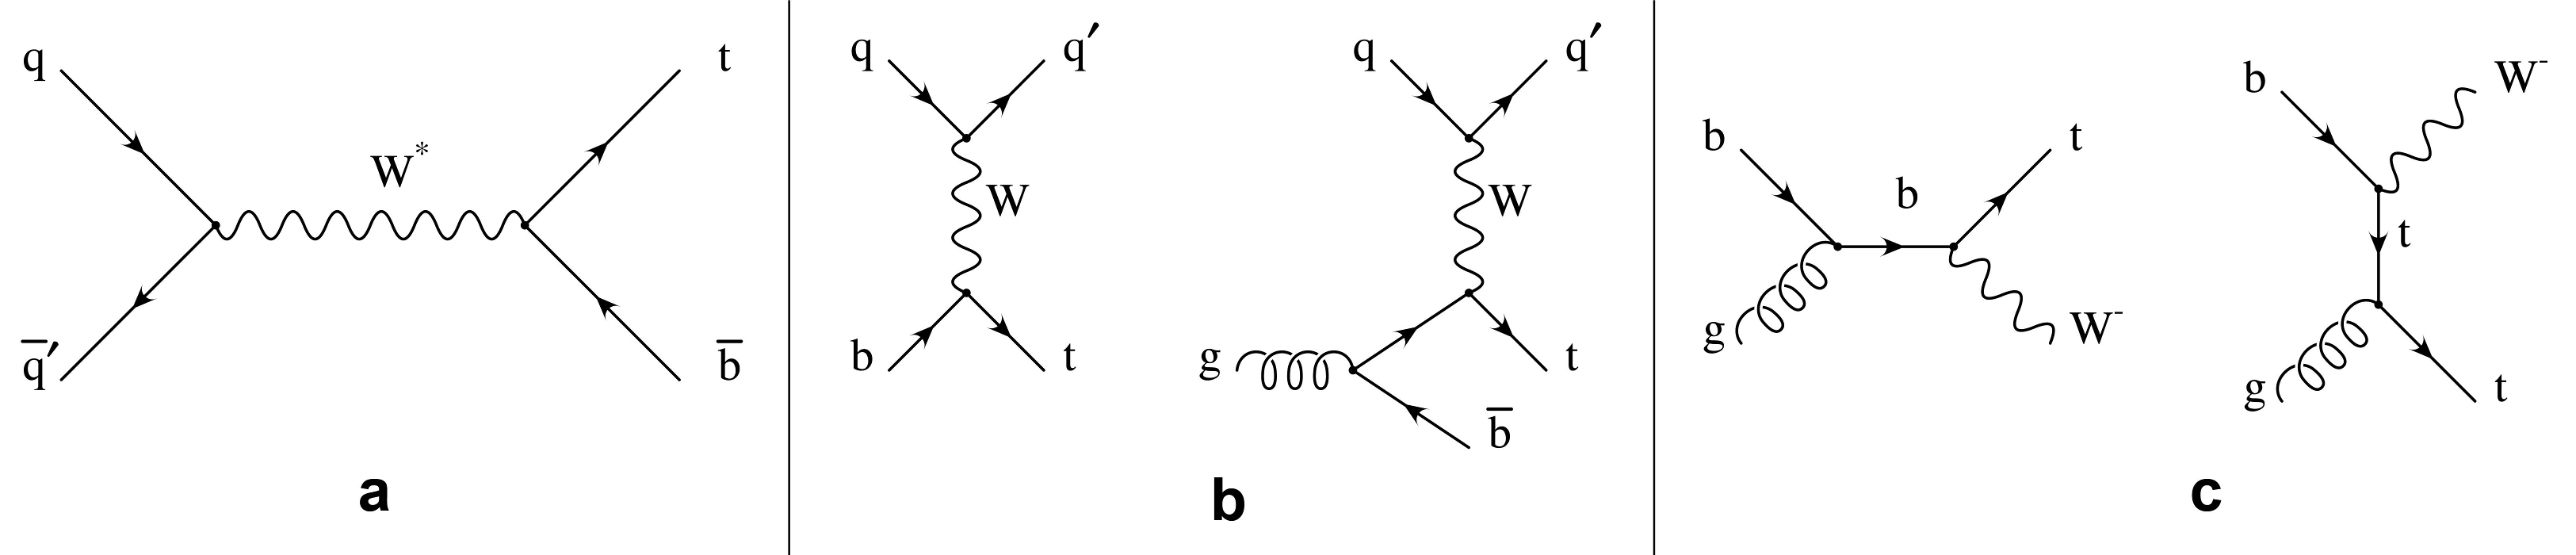
\includegraphics[width=1.\textwidth]{img/singletop}
    \caption[Produktionskanäle für ein einzelnes Top-Quark in Proton-Proton
        Kollisionen]
        {Produktion eines einzelnen Top-Quarks in Proton-Proton Kollisionen im
        s-Kanal (a), t-Kanal(b) und mit einem W-Boson im Ausgangszustand (c).}
    \label{fig:singletop}
\end{figure}

Für die Produktion im t-Kanal (b) wurde für den harten Prozess \textsc{AcerMC}
(\cite{Kersevan:2004yg}) als Generator verwendet, der eine Schnittstelle zu
\textsc{Pythia6} (\cite{1126-6708-2006-05-026}) zur Simulation von
Bremsstrahlung und Hadronisierung bereitstellt. Die beiden anderen Kanäle und
die Produktion eines Top-Paares wurden hingegen mit \textsc{MC@NLO}
(\cite{Frixione:2002ik}) simuliert, ein Generator, der neben dem harten Prozess
auch die Hadronisierung beschreibt.






%______________________________________________________________________________
%                                                                     Selektion 
\section{Selektion}
\label{data_sim_selection:selection}

\begin{itemize}
    \item Motivation für Schnitte (Untergrund-Diskriminierung)
    \item Event-basierte Schnitte (Trigger, Detektor, primVertex)
    \item Elektron-basierte Schnitte (CC/CF, pT, ID, Autor, IQ)
    \item kurze erwähnung andere schnitte (MET,Jets,...)
\end{itemize}


